\newif\ifshowsolutions
\showsolutionstrue

\documentclass{article}
\usepackage{algorithm,algpseudocode}
\usepackage{listings}
\usepackage{amsmath}
%\usepackage{subfigure}
\usepackage{subfig}
\usepackage{amsthm}
\usepackage{amsmath}
\usepackage{amssymb}
\usepackage{graphicx}
\usepackage{mdwlist}
\usepackage[colorlinks=true]{hyperref}
\usepackage{geometry}
\usepackage{titlesec}
\geometry{margin=1in}
\geometry{headheight=2in}
\geometry{top=2in}
\usepackage{palatino}
\usepackage{mathrsfs}
\usepackage{fancyhdr}
\usepackage{paralist}
\usepackage{todonotes}
\setlength{\marginparwidth}{2.15cm}
\usepackage{tikz}
\usetikzlibrary{positioning,shapes,backgrounds}
\usepackage{float} % Place figures where you ACTUALLY want it
\usepackage{comment} % a hack to toggle sections
\usepackage{ifthen}
\usepackage{mdframed}
\usepackage{verbatim}
\usepackage[strings]{underscore}
\usepackage{listings}
\usepackage{bbm}
\rhead{}
\lhead{}

\renewcommand{\baselinestretch}{1.15}

% Shortcuts for commonly used operators
\newcommand{\E}{\mathbb{E}}
\newcommand{\Var}{\operatorname{Var}}
\newcommand{\Cov}{\operatorname{Cov}}
\newcommand{\Bias}{\operatorname{Bias}}
\DeclareMathOperator{\argmin}{arg\,min}
\DeclareMathOperator{\argmax}{arg\,max}

% do not number subsection and below
\setcounter{secnumdepth}{1}

% custom format subsection
\titleformat*{\subsection}{\large\bfseries}

% set up the \question shortcut
\newcounter{question}[section]
\newenvironment{question}[1][]
  {\refstepcounter{question}\par\addvspace{1em}\textbf{Question~\Alph{question}\!
    \ifthenelse{\equal{#1}{}}{}{ [#1 points]}: }}
    {\par\vspace{\baselineskip}}

\newcounter{subquestion}[question]
\newenvironment{subquestion}[1][]
  {\refstepcounter{subquestion}\par\medskip\textbf{\roman{subquestion}.\!
    \ifthenelse{\equal{#1}{}}{}{ [#1 points]:}} }
  {\par\addvspace{\baselineskip}}

\titlespacing\section{0pt}{12pt plus 2pt minus 2pt}{0pt plus 2pt minus 2pt}
\titlespacing\subsection{0pt}{12pt plus 4pt minus 2pt}{0pt plus 2pt minus 2pt}
\titlespacing\subsubsection{0pt}{12pt plus 4pt minus 2pt}{0pt plus 2pt minus 2pt}


\newenvironment{hint}[1][]
  {\begin{em}\textbf{Hint: }}{\end{em}}

\ifshowsolutions
  \newenvironment{solution}[1][]
    {\par\medskip \begin{mdframed}\textbf{Solution~\Alph{question}#1:} \begin{em}}
    {\end{em}\medskip\end{mdframed}\medskip}
  \newenvironment{subsolution}[1][]
    {\par\medskip \begin{mdframed}\textbf{Solution~\Alph{question}#1.\roman{subquestion}:} \begin{em}}
    {\end{em}\medskip\end{mdframed}\medskip}
\else
  \excludecomment{solution}
  \excludecomment{subsolution}
\fi

\usepackage{xcolor} % Required for specifying custom colors
\usepackage{fix-cm} % Allows increasing the font size of specific fonts beyond LaTeX default specifications

\setlength{\oddsidemargin}{0mm} % Adjust margins to center the colored title box
\setlength{\evensidemargin}{0mm} % Margins on even pages - only necessary if adding more content to this template

\newcommand{\HRule}[1]{\hfill \rule{0.2\linewidth}{#1}} % Horizontal rule at the bottom of the page, adjust width here

\definecolor{grey}{rgb}{0.9,0.9,0.9} % Color of the box surrounding the title - these values can be changed to give the box a different color	
\newcommand{\boldline}[1]{\underline{\textbf{#1}}}

\chead{%
  {\vbox{%
      \vspace{2mm}
      \large
      Network Economics \hfill
      Caltech CS/EE/144 \hfill \\[1pt]
      Miniproject 1\hfill
      Team RankBeaver \\
    }
  }
}

\begin{document}
\pagestyle{fancy}
\begin{titlepage}
\parbox[t]{1.0\linewidth}{
	\centering \fontsize{50pt}{80pt}\selectfont % The first argument for fontsize is the font size of the text and the second is the line spacing - you may need to play with these for your particular title
	\vspace*{0.7cm} % Space between the start of the title and the top of the grey box
		
	\hfill \center{Rankmaniac Report}\\
	\vspace*{0.7cm} % Space between the end of the title and the bottom of the grey box
}

%----------------------------------------------------------------------------------------
{\centering \large 
\hfill Team RankBeaver
} \\

\vfill % Space between the title box and author information

%----------------------------------------------------------------------------------------
%	AUTHOR NAME AND INFORMATION SECTION
%----------------------------------------------------------------------------------------

{\centering \large 
\hfill Xinjie Lei, Jian Zhu, Tianlei Sun, Hongnian Yu \\
\hfill California Institute of Technology \\
\hfill Department of Electrical Engineering \\

\HRule{1pt}} % Horizontal line, thickness changed here

%----------------------------------------------------------------------------------------

\clearpage % Whitespace to the end of the page
\end{titlepage}

\section{Team Member \& Work Split}
\medskip
\begin{itemize}

    \item \boldline{Group members} \\
    Xinjie Lei\\
    Tianlei Sun\\
    Hongnian Yu\\
    Jian Zhu
    
    \item \boldline{Team name} \\
    RankBeaver
    
    \item \boldline{Division of labour} \\
    Xinjie Lei: Implemented the PageRank reduce algorithm, helped in debugging PageRank map algorithm, explored ways of optimizing code structure, and brainstormed for speed optimization.\\
    Tianlei Sun: Coordinated and debugged different modules, optimized the Neighbor List Algorithm, researched and implemented Top K Page Rank method.\\
    Hongnian Yu: Implemented the page rank mapper algorithm, helped debug page rank reducer program, searched paper online and brainstormed for speed optimization.\\
    Jian Zhu: Implemented the processor algorithm, helped debug page rank reducer program, and collaborated in optimizing the Top K Page Rank method.

\end{itemize}



\section{Introduction}
\medskip
\begin{itemize}

    \begin{figure}[H]
    \centering
    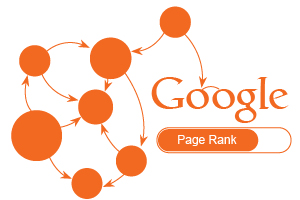
\includegraphics[width=11cm,height=6cm]{intro_img.jpg}
   	%\caption{Insert caption here.}
    \end{figure}
\item Page Rank is an algorithm for measuring the importance of pages in a web graph. It is developed by Larry Page and Sergey Brin in 1996, and later adopted by Google for its initial prototype search engine. The algorithm takes in representation of a web graph (adjacency List, adjacency matrix, etc..) and output the probability distribution for different web pages. The details of page rank algorithm is given as follows:\[ G=\alpha*P+\frac{(1-\alpha)}{n}*\mathbbm{1},\]\[ r(t) = r(t-1)*G \]\\n is the total number of vertex in the graph, and alpha is the damping factor, P is the transition matrix, r(t) is the page rank vector at iteration t. We initialize r(0) to be 1/n, and multiply it by G at each iteration.\\The map reduce framework comes into place if we realize that the page rank of node i at iteration t, denoted as r(t)[i], is only determined by the transition matrix and page rank vector at the previous iteration. Therefore, we can calculate the page rank of different node at iteration t in parallel. Moreover, considering r(t)[i]=r(t-1)*column i of G, this computation process is equivalent to summing up all the contributions to node i from all the node which are connected to i. In this way, we no longer need to deal with matrix form multiplication. The implementation details can be found in the algorithm section below.

\end{itemize}



\section{Original Algorithm}
\medskip
\begin{itemize}

    \item \boldline{Mapper Algorithm}
    \begin{itemize}
    % Insert text here. Bullet points can be made using '\item'.
    \item \textbf{Pseudo code:}
    
    \begin{minipage}{\linewidth}
    \begin{algorithm}[H]
    \caption{Mapper algorithm}\label{process}
    \begin{algorithmic}[1]
    \Procedure{mapper}{$std\_input$}\Comment{mapper actual input is inside std\_input}
    \State $(nodeID, iteration, currRank, neighborsList)\gets parse\, std\_input$    
    \For{$neighbor$ in neighborsList}
    \State$individualScore \gets\alpha * currRank/length\,of\, neighborsList$
    \State $std\_out.write($neighbor, individualScore$)$
    \EndFor
    \State $std\_out.write($nodeID,iteration,neighborsList$)$
    \EndProcedure
    \end{algorithmic}
    \end{algorithm}
    \end{minipage} \\[1em]
    
    
    
    
    
    
    
    \item \textbf{Explanation:}\\
    The mapper function first read and parse std input. Then we calculate the individual score based on the formula \(individual\ score = \alpha * currRank / out\_degree \). Individual score means the contribution of node i to its neighbor j for j's page rank in the current iteration. We emit neighborID and contribution. This contribution is later collected by collectors and group by key(neighbor's id) to determine the neighbor node's page rank in the current iteration. In addition to individual score. We also need to emit nodeID, iteration number, and its neighborsList so that the process reducer can keep track of the current iteration number and not lose the graph information(nodeID and neighborsList). To improve efficiency, this information only need to be emit once.
    \end{itemize}


    \item \boldline{Reducer Algorithm}
    \begin{itemize}
    \item \textbf{Pseudo Code:}\\
    \begin{minipage}{\linewidth}
    \begin{algorithm}[H]
    \caption{Reducer algorithm}\label{process}
    \begin{algorithmic}[1]
    \Procedure{reduce}{}
    \State$key \gets $None
    \State$rankContributions \gets $\{\}
    \For{$line$ in std\_in}
    \State$nodeID, oneContribution, iteration, neighborsList \gets$ parse($line$)
    \If{key is None}
    \State $key \gets $nodeID
    \ElsIf{$key \neq $nodeID}
        \State$rank \gets$ sum($rankContributions$) + 1 - \(\alpha\) 
        \State std\_out.write($nodeID, rank, iteration, neighborsList$)
        \State $rankContributions \gets $\{\}
        \State $key \gets $nodeID 
    \EndIf
    \State append $oneContribution$ to $rankContributions$
    \EndFor
    \EndProcedure
    \end{algorithmic}
    \end{algorithm}
    \end{minipage} \\[1em]

    \item \textbf{Explanation:}\\
    Based on the PageRank algorithm, we derived the following formula for PageRank of an individual node,
    \[r(t)_{i,j} = \alpha * r(t-1)_{i, *} * P_{*, j} + n * \frac{1-\alpha}{n} =  \alpha * r(t-1)_{i, *} * P_{*, j} + 1 - \alpha\]
    The mapper already emits \(r(t-1)_{i, *} * P_{*, j}\) element-by-element in a sequence. The collector groups them and sends the sequence to the reducer. Thus, the reducer only needs to sum up the PageRank contributions from all neighbors of key(node id),  multiply the sum with the damping factor \(\alpha\) and add the result with \(1 - \alpha\) which guarantees an aperiodic and strongly-connected graph.

    \end{itemize}
    
    \item \boldline{Processor Algorithm}
    \begin{itemize}
    % Insert text here. Bullet points can be made using '\item'.
    \item \textbf{Pseudo Code:}\\
        \begin{minipage}{\linewidth}
        \begin{algorithm}[H]
        \caption{Processor algorithm}\label{process}
        \begin{algorithmic}[1]
        \Procedure{process}{}
        \State $topRank \gets \{\} $
        \For{$line$ in std\_in}
        \State $nodeID, rank, iteration, neighborsList \gets$ parse($line$)
        \If{$iteration <$ MAX_ITR}\Comment{More iterations to go}
            \State std\_out.write($nodeID, rank, iteration, neighborsList$)
        \Else
            \While{length$(topRank) <20$}\Comment{use heap sort to find the top 20 ranks}
                \State add $(nodeID, rank)$ to $topRank$
            \EndWhile
            \State $(id, minVal) \gets \min(topRank)$
            \If{$rank > minVal$}
                \State delete $(id, minVal)$ from $topRank$
                \State add $(nodeID, rank)$ to $topRank$
            \EndIf
        \EndIf
        \EndFor
        \State sort the top 20 ranks
        \EndProcedure
        \end{algorithmic}
        \end{algorithm}
        \end{minipage} \\[1em]
    
    \item \textbf{Explanation:} The processing part is executed after mapping and reducing. It takes the output from the reducer algorithm and decide whether to proceed to another iteration or output the final results. If the maximal iteration which is set manually has not been reached yet, it will parse the input to the format that can be read by the mapper. Otherwise it will use heap sort to find the top 20 ranks and then sort them in descending order as the output.
    \end{itemize}

\end{itemize}



\section{Optimization}
\medskip
\begin{itemize}
    \item \boldline{Code Structure Optimization:}\\
    We considered following code structure optimizations:
    \begin{itemize}
    \item Avoid unnecessary string conversion: For variables node id, iterations, and neighbor lists, we converted them to integers only when the variables participated in computations. Otherwise, we used string format of the variables for branching. This optimization improved the performance in a limited extent.
    \item Avoid unnecessary list join: PageRank mapper receives neighbor node list for each node and passes it to the reducer. In the original code, we split the neighbor list string to a list and then joined the list to a new string as part of the standard output. This operation was inefficient because the large amount of nodes in test data set would introduce repetitive split and join in each iteration. Thus, we kept the neighbor list string and created a new list variable holding the string splitting result to improve the overall long-run performance.
    \item Use regular expression for string parsing: We used several string splitting function calls in the initial line parsing method which created multiple unnecessary temporary lists. To improve the speed and memory utilization, we adopted regular expressions to parse the standard input considered the flexibility and conciseness of regular expressions. However, overall performance was worsen because of the inner greedy algorithm regular expression used to match a pre-defined pattern. Thus, we abandoned the regular expressions and stuck on string splitting instead.
    \end{itemize}
    
    \item \boldline{Neighbor List Optimization:}\\
    The main function of the Pagerank reducer part is to sum up the PageRank contributions from each nodes. However, it's also important to pass the neighbor list to the next iteration. In the beginning, we planed to attach the neighbor list at the back of each mapper emit. However, this is every inefficient because we only need one copy neighbor list for each node, while this method provide redundant copies of the neighbor list. Therefore, we brainstormed a new way with two different form of mapper output and reducer input:
    \begin{enumerate}
        \item NodeID -tab- value
        \item NodeID -tab- iteration, neighbor list
    \end{enumerate}
    The first form appears in each mention in neighbor list, but the second form appears once once. The reducer recognizes the two different formats, sums the values for each NodeID and output one result for each NodeID:
    \begin{enumerate}
        \item NodeID -tab- sum, iteration, neighbor list
    \end{enumerate}
    This method dramatically increases the performance and helped us exceeds the milestone performance.
    
    
    \item \boldline{Top K page rank Optimization -- An interesting failure attempt:}\\
    \begin{itemize}
        \item \textbf{Implementation: }  After we pass the milestones, our next approach is to sacrifice accuracy for speed. We plan to reduce the time cost of each iteration. And our approach is to cut the unnecessary nodes affected by [1].\\
        
        \begin{minipage}{\linewidth}
        \begin{algorithm}[H]
        \caption{Top K page rank algorithm}\label{euclid}
        \begin{algorithmic}[1]
        \Procedure{node cutting}{$graphList, K$}\Comment{graphlist is a list of all nodes}
        \State $n\gets length(graphList)$
        \For{$node \text{ in } graphList$}
         \If{$node\text{'s rank is in top K}$}
         \State $topKlist \text{ appends } node$\Comment{Nodes in topK_list won't be cut}
         \EndIf
        \EndFor
        \State $finalList \gets topKlist$
        \For{$node \text{ in } topKlist$}
         \For{$supportNode \text{ in } node \text{'s neighbor list} $}
          \If{$node\text{'s rank is in top K}$}
          \State $finalList \text{ appends } supportNode$\Comment{support Nodes of topK_list won't be cut}
          \EndIf
         \EndFor
        \EndFor
        \State \textbf{return} $finalList$\Comment{return the top K nodes and their support nodes}
        \EndProcedure
        \end{algorithmic}
        \end{algorithm}
        \end{minipage}\\[1em]
        
        \item \textbf{Result: }  This algorithm can reduce 50$\%$ of time cost in each iteration according to our local test. But unlucky, the high penalty of the AWS overhead(5min each iteration) means that the actual runtime of each iteration is only about 1min and thus there is no help in reducing time for each. We sadly find out that the only effective way is to reduce the number of iterations and predict the result.
        
    \end{itemize}
\end{itemize}



\section{Conclusion}
\medskip
\begin{itemize}

    \item \boldline{Discoveries} \\
    % Insert text here.
    In this project we implemented MapReduce to compute the ranks of nodes in a graph based on the transition matrix. We realized that it could be time-consuming to iterate over the transition matrix until it converges, so stopping criterion and optimization on the computation process would be meaningful. We found that generally it will converge after a dozen times, so reducing the number of iterations or the running time in each iteration would make the process much more efficient. We tried the method of optimizing the page rank algorithm and found it effective in lower the time cost of each iteration. However, due to the AWS overhead, the progress was not so dictinct in practice.

    \item \boldline{Challenges} \\
    % Insert text here.
    The main challenge was that our optimization was limited by the overhead in each iteration. Our attempt in optimization was effective in the local test, but we did not realize the overhead issue. Stuggling with decreasing time cost in each iteration instead of reducing iterations proved to be not so effective in AWS although we tried multiple methods in optimizing our algorithm.

    \item \boldline{Future Improvement} \\
    % Insert text here.
    We would consider reducing the number of iterations to optimize our algorithm. This is more pratical regarding the overhead in each iteration. By setting some stopping criterion and predicting principle we can terminate the computation process earlier and predict the final ranks with enough accuracy. This would be much more beneficial if we take the actual running cost into consideration.
\end{itemize}

\section{References}
\begin{enumerate}
    \item[] [1]. Fujiwara, Y., Nakatsuji, M., Shiokawa, H., Mishima, T., Onizuka, M. (2013, July). Fast and Exact Top-k Algorithm for PageRank. In AAAI.
\end{enumerate}

\end{document}